% Activate the following line by filling in the right side. If for example the name of the root file is Main.tex, write
% "...root = Main.tex" if the chapter file is in the same directory, and "...root = ../Main.tex" if the chapter is in a subdirectory.
 
%!TEX root =  mainMastersProject.tex

\chapter[Simple Non-Spatial Simulations]{A Simple Stabbing - Non-Spatial Simulations and their Bayesian Networks}

\section{Introduction}
Here I talk about the credibility game and Charlotte Vlek's Stabbing Bayesian Network example.

In these non-spatial simulations, there are agents, and they interact with each other, but there is no environment for them to interact in. So the simulation is a pure combination of the probabilities assigned to each state transition (or something along those lines). In a sense, the probability for an agent to `stab with knife' purely depends on the probability of `motive' and `opportunity'. Compared to a spatial simulation, where `opportunity' is more complex, as it involves proximity to victim which arises from the simulation and not from some random number generator.

These non-spatial simulations are boring, but they are necessary first steps: after all, if we cannot make BNs out of these predetermined (the probabilities in each run are not predetermined, but the distributions that they are drawn from, and their thresholds, are), then the rest of our endeavours will be fruitless. On the other hand, if the process for creating and evaluating these simple simulations work well, then we can proceed to modelling more complex, spatial simulations.

In this part, I have two experiments. One simple experiment meant to be a replication of Charlotte Vlek's Bayesian Network in xxx \footnote{rephrase}, and another simple experiment mainly meant to test the evaluation criteria for the Bayesian Networks, as outlined in the previous chapter.

\section{Method}
%There are two methods outlined here, one for each initial experiment.

Take the Vlek networks from Vlek Jurix 2015.

The general story is: Jane and Mark had a fight, but Jane had a knife. Mark died. 

Then, there are two specific scenarios that can explain why Mark died. In scenario one, Jane stabbed Mark, and then he died. In scenario 2, Jane threatened Mark with the knife, Mark hit Jane, Jane dropped the knife, Mark fell on the knife, and Mark died by accident. There are two separate networks for these scenarios.

I'm going to create two separate networks, and then also see if I can merge them, by creating a Jane-and-Mark-knife simulation, assigning some random probabilities that correspond to the story, and see what the K2 algorithm makes of it. Then I will also merge the two networks to see if the K2 can deal with mutually exclusive nodes (eg: `Mark died by accident' should rule out `Mark died by stabbing').

So, I created some logical rules, either atoms or rules, and we can process in the simulation these using standard forward chaining inference. Every atom has a prior probability, and every conclusion of a rule has a probability given the F/T state of the premises. At every step, the simulation checks which new sentences are true, applies a rule with a given probability, and counts the outcome.

This does mean that rules at the end are not triggered as often as rules in the beginning, even if they have the same trigger probability (they are on other sides of the chain, more needs to be have happened to conclude that Mark died).

\subsection{Behavioural rules for the simulation}

\begin{table}
\begin{tabular}{|c|c|c|}
 \hline
 Premise & Conclusion & P(conclusion) given premises\\
 \hline
  & Jane and Mark fight   & 20   \\
  & Jane has knife & 70 \\
  \color{blue}Jane and Mark fight, Jane has a knife & Jane stabs Mark with knife & 1 \\
 \color{red}Jane and Mark fight, Jane has a knife & Jane threatens Mark with knife & 3 \\
  \color{red}Jane threatens Mark with knife & Mark hits Jane & 90 \\
  \color{red}Mark hits Jane & Jane drops knife & 50  \\
  \color{red}Jane drops knife & Mark falls on knife & 10 \\
  \color{red} Mark falls on knife & Mark dies by accident & 60  \\
  \color{blue}Jane stabs Mark with knife & Mark dies  & 70 \\ 
  \color{red}Mark dies by accident & Mark dies & 100  \\ 
\hline
\end{tabular}
\caption{For combined scenarios: blue rules belong to scenario 1, red rules belong to scenario 2, and black rules belong to both.}
\end{table}

This was done using forward chaining, with a time index, which means that a rule could only be triggered at one time (otherwise the probabilities get messed up). So we have a forward chaining rule, which means that if the premises of some rule are true, there are no excluding facts true, the timestep is correct, and the random number generator generated a number that is lower than the probability threshold, we find that the conclusion is true, and add it to our found facts. We keep doing this.

Vlek's paper contains no probabilities, so I'm just making some up. The logical sentences are reporters in the simulation, and then I let the simulation run for 10,000 times. 

\section{Results}
We succeeded in generating three different BNs:  One for scenario 1, one for scenario 2, and one for the combined network (Figure~\ref{kb1}, Figure~\ref{kb2}, Figure~\ref{full}).

\begin{figure}[htbp]
\begin{center}
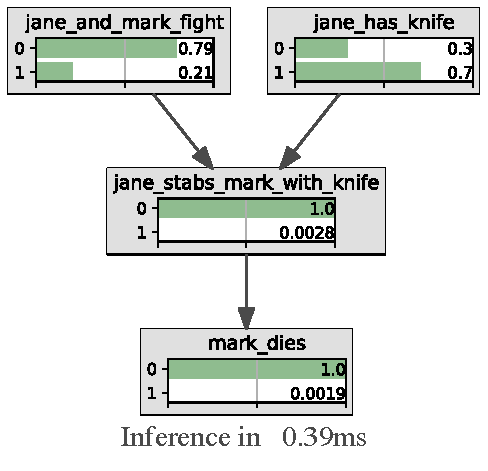
\includegraphics[]{images/Kb1.pdf}
\caption{Automatically generated BN with K2 and the above forward chaining rules, scenario 1.}
\label{kb1}
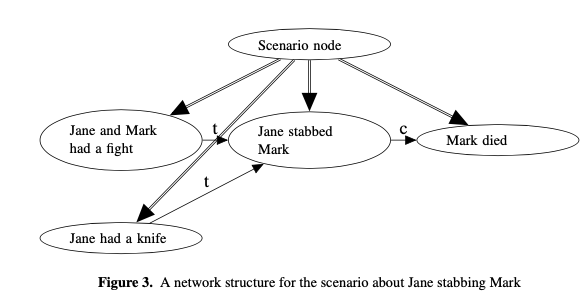
\includegraphics[scale=0.55]{images/vlek2015a.png}
\caption{Vlek BN.}
\label{vlek1}
\end{center}
\end{figure}


\begin{figure}[htbp]
\centering
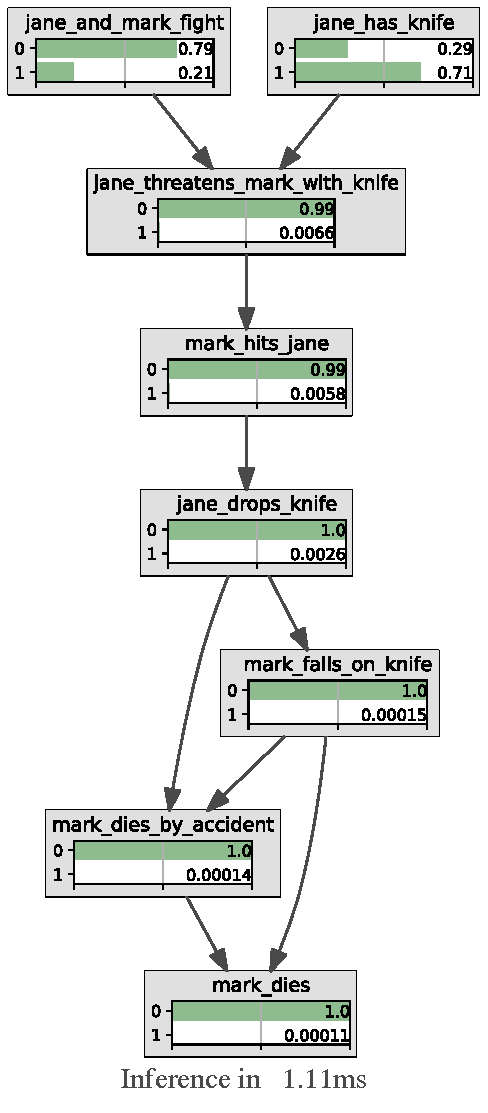
\includegraphics[scale=0.7]{images/Kb2.pdf}
\caption{Automatic generated BN with K2 and above forward chaining rules, scenario 2}
\label{kb2}
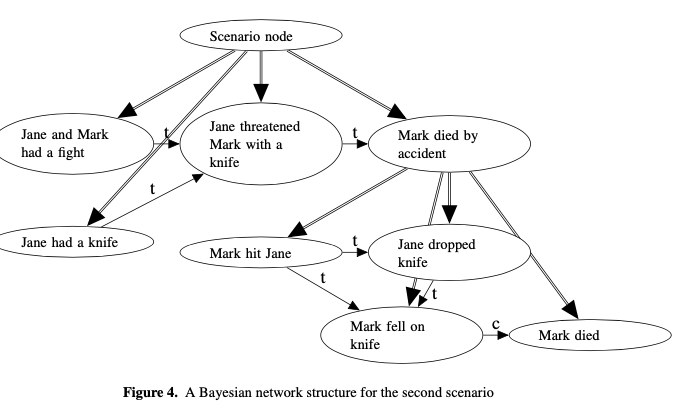
\includegraphics[scale=0.55]{images/vlek2015.png}
\caption{Vlek BN.}
\label{vlek}
\end{figure}


\begin{figure}[htbp]
\begin{center}
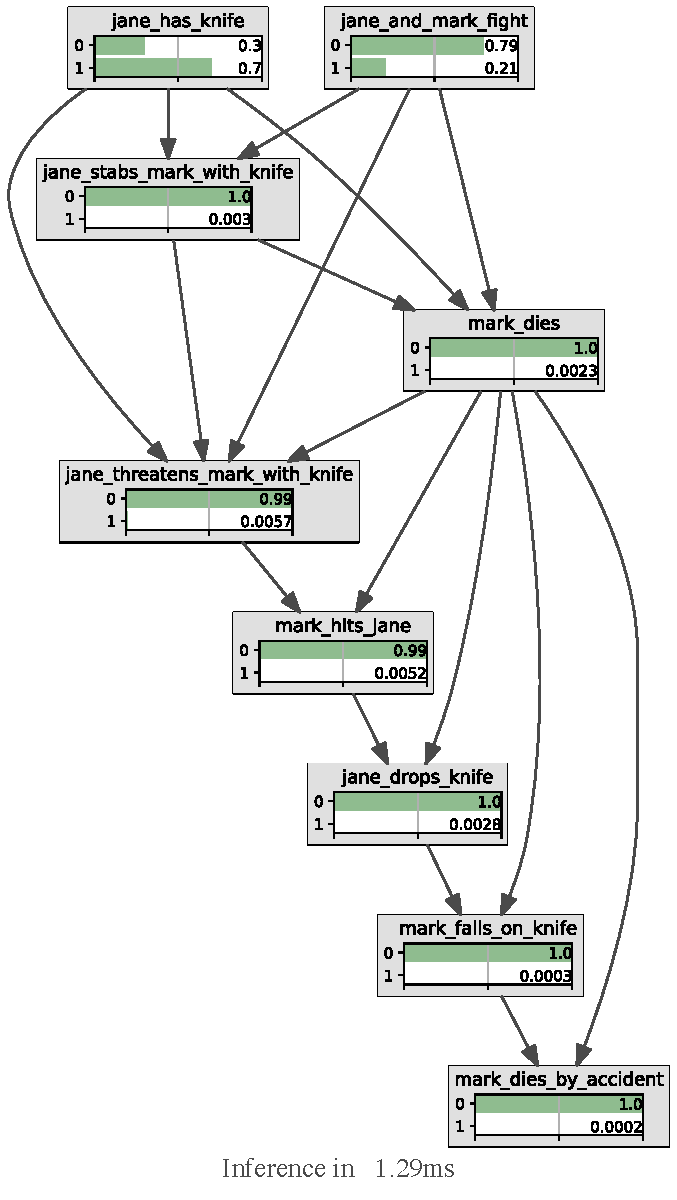
\includegraphics[scale=0.8]{images/Kb.pdf}
\caption{Automatically generated BN with rules from both scenarios included.}
\label{full}
\end{center}
\end{figure}

\section{Discussion}
How well do these networks evaluate compared to the criteria we set out initially, and how well do they compare to the Vlek networks, and the criteria set out in Vlek 2015?




\subsection{Structural Criteria}
\begin{enumerate}
\item (temp) Events are ordered temporally - scenario-like.

In the forward chaining knowledge base, we have premises and conclusions. If we take the event in a conclusion, then we know that the premise of that rule, is the parent of that node in the Bayesian Network. (again, rephrase this is so vague. Maybe make it a rule or smth). The two ``premiseless'' events Jane and Mark fight, and Jane has a knife, are also parentless in the simulation. In this sense, the structure of the Bayesian Network reflects the structure of the inference rules that we set out.

We see that in both the separate networks, the temporal ordering of the nodes is correct - every node has as a parent a node that represents an event that would have happened beforehand. In the combined network, this is not the case: mostly the temporal links are represented ok (eg: the chain of events from "Jane threatening Mark" to "Mark dies by accident" is represented correctly), however, this chain of nodes all has as a parent "Mark dies", which would, temporally, occur only after "Mark falls on knife" occurs. This means that in the combined Bayesian Network, we cannot satisfy the temporal ordering constraint due to the conditional probabilities between the events (eg: if Jane stabs Mark, then she cannot threaten him after, which is a relation that `inhibits' the `Jane threatening Mark' node - eg: there is a conditional relation between the two nodes, but not a temporal or causal one). As a conclusion about this criteria: Maybe temporal ordering should just hold within scenarios and not between scenarios, because we get into these sorts of causal messes. Or we should use the scenario node to organise different scenarios together. Idea: scenario node could cause temporal ordering, but what in cases with much shared evidence?

\item (con) Evidence connects to hypotheses.

In the original network, we have no evidence, so it is not included into this one. However, I might add some evidence to test the Performance Criteria.

\item (exc) All events that are irrelevant are not included in the scenario BN.

This criteria, and the next one, are freebies, because we are just copying a network that already exist - our set of relevant events is the same as that in the original network by Vlek. We do not have any irrelevant event because we can see that all events are connected to each other, and all events reflect an underlying `decision' by an agent.

\item (exh) All events that are relevant are included in the scenario BN.

We have included all relevant events - all the events in the knowledge base are also in the network.

\item (ind) Independent events are not connected to each other.

This is not entirely correct in the uncombined networks (and also not correct in the combined network) - If Mark dies by accident, this is only dependent on Mark falling on the knife, and not also on Jane dropping the knife (since all cases where Mark dies by accident are also cases where Mark falls on the knife, we don't need a separate condition for Jane dropping the knife). This is probably due to an insufficient number of runs (eg: the probability that this happens is very low and we might not have enough data to correctly estimate it).


\end{enumerate}

\subsection{Performance Criteria}


\begin{enumerate}
\item The accuracy of the network is not lower than the inherent randomness of the simulation.



\item The strong and the weak view.

The strong view: probabilities in the network correspond exactly to probabilities in the simulation. The weak view: Updates on evidence in the network go in the same direction as updates on evidence in the simulation.

\begin{table}
\begin{tabular}{|c|c|c|}
 \hline
 Conclusion &P(conclusion) given premises & P(event) given premises\\
 \hline
 Jane and Mark fight   & 20 &  20.87   \\
 Jane has knife & 70 & 70.23 \\
 Jane stabs Mark with knife & 1 & 2.05 \\
 Mark dies & 70 & 75.46 \\ 
\hline
\end{tabular}
\caption{For only scenario 1.}

\begin{tabular}{|c|c|c|}
 \hline
 Conclusion &P(conclusion) given premises & P(event) given premises\\
 \hline
 Jane and Mark fight   & 20 &  20.87   \\
 Jane has knife & 70 & 70.23 \\
 Jane threatens Mark with knife & 3 & 3.88 \\
 Mark hits Jane & 90 & 90.21 \\
 Jane drops knife & 50 & 50.09 \\
 Mark falls on knife & 10 & 11.13\\
 Mark dies by accident & 60 & 61.25 \\
 Mark dies & 100 & 99.79 \\ 
\hline
\end{tabular}
\caption{For only scenario 2}
\end{table}

For both scenarios, the probabilities in the network are very similar to the probabilities in the ground truth (simulation). There is a
loss of precision, which is the worst in case of `Mark dies' in the first scenario, which is estimated at 75\% by the network, but in fact in the simulation is only 70\% probable. I don't know where this comes from. Apart from that, all divergences for the original probabilities are within 2\%. This means the strong view does not hold, but the weak view does (updating on evidence gets us with probabilities that are closer to the simulation probabilities than before).


\begin{table}
\begin{tabular}{|c|c|c|}
 \hline
 Conclusion &P(conclusion) given premises & P(event) given premises\\
 \hline
 Jane and Mark fight   & 20 &  20.87   \\
 Jane has knife & 70 & 70.17 \\
 Jane stabs Mark with knife & 1 & 2.06 \\
 Jane threatens Mark with knife & 3 & 3.88 \\
 Mark hits Jane & 90 & 91.50 \\
 Jane drops knife & 50 & 52.97 \\
 Mark falls on knife & 10 & 10.92\\
 Mark dies by accident & 60 & 66.33 \\
 Mark dies (premise: Jane stabs Mark) & 70 & 68.68 \\ 
  Mark dies (premise: Mark dies by accident)& 100 & 98.77 \\ 
\hline
\end{tabular}
\caption{For combined scenarios}
\end{table}

The probabilities of the conclusions in the combined network given the premises, also look relatively similar on a human scale - I assume that a human probability elicitor would not be able to distinguish between a probability of 11.13, 10.92 or 10.00 for the conclusion ``Mark falls on knife". On the other hand, if we round all the probabilities in the network to 10, a human probability elicitor might be able to say that the probability of `Mark falls on knife'' is 0.1 (or 10\%), to exactly that level of precision (so not 0.10, or 0.100). The resulting probabilities might be elicitable, while still meaningfully reflecting the ground truth.


\item Sensitivity analysis shows that no simulation-irrelevant event influences some output \footnote{rephrase}
\end{enumerate}

\subsection{Human Criteria}
\begin{enumerate}
\item Do we think that a human can find these numbers?

The conditional probability tables as displayed in these networks are not great.

	\begin{enumerate}
	\item How robust is the network against disturbances around the mean (problem with precision)?
	\item How robust is the network around rounding to arbitrary intervals?
	\end{enumerate}
\end{enumerate}




\subsection{Comparison to Vlek 2015}
If we only look at the ordering of the Bayesian Network, we can see that for Figure~\ref{kb1}, the sub-scenario structure is the same as in Vlek 2015 Figure~3, our Figure~\ref{vlek1}. There's no scenario node constraining the network, all the information is contained in the network, no scenario node needed (todo: make the nodes the exact same names).

However, there are differences between Vlek 2015 Figure~4, and the automatically generated BN here. Figure~4 in Vlek 2015 is replicated below in Figure~\ref{vlek} (todo: ask permission?? or just remove). The automatically generated BN is very linear and can be interpreted in a purely temporal way: mark hits jane, jane drops the knife, and due to jane dropping the knife, and mark falling on it, mark dies by accident - and if mark dies by accident, mark dies. The probabilities for all these events (from jane dropping the knife on), are ridiculously low, and don't really make sense (should interpret the small probabilities as e, and not as actual numbers I guess, due to underflow?). 

In Vlek's paper, we see a subscenario: we have the subscenario ``Mark died by accident", which contains events such like mark hit jane, which leads to jane dropping the knife, and mark falling on the knife, and then dying. The coparents of Mark died are the same in this network as in the automatically generated BN, however, we once-again miss the scenario-like construction where mark hitting jane, jane dropping the knife, and mark falling on the knife are connected as part of a subscenario, rather than their ``own" nodes.


Why to choose for subscenarios when it is not required? Tomorrow I will look up why the scenario construction was used and I will see if it does something that I miss? Coherence? But that also travels up the chain? But something with d-separation probably. I'll read the Vlek 2015 again i guess.



In the full final network, we see that the two mutually exclusive scenarios (stabbing vs falling on knife) are excluding each other even without the use of a scenario node - so we can make networks that combine two different stories. This is nice.

\subsection{Quality of scenario}
\begin{itemize}
\item Completeness - have all the parts and not one more. Not a big deal for this simulation, as I've taken all the nodes from Vlek 2015, there's no discussion about granularity.

\item Consistent - no internal contradictions. There is no explicit structure in the final BN that ensures consistency. The probabilities inside the BN need to ensure that. For instance, the only thing that is contradictory in the KB is that jane threatening and jane stabbing, cannot both happen. In the final network (Figure~\ref{full}), there are nodes for both threatening and stabbing. However, the relations of these nodes are such, that when one node becomes more likely (eg, we set evidence on it),  the other node becomes less likely (as we can see in the figure below:

figure here of $\Delta$ P stabbing for increasing values of P threatening. If we know threatening is true, stabbing goes to 0, and vice-versa - and all the consequences of the threatening scenario also go to 0, so it just works. This means that several different scenarios can be combined into one network, and still be mutually exclusive. Both scenarios share some events (as some scenarios can do in real life), but the different scenarios themselves are not separated from each other by structure or construction (as is the case in Vlek~2015).

Do we need the constraint node? Or do we only use that if we have knowledge but no data? what. 11 in Vlek.

We can just straight-up draw a line between two events in order for them to become mutually exclusive, like we do with Jane stabs mark and jane threatens mark. Fenton et al advice against that - we draw a relation between two causes to ensure mutual exclusivity. Fenton doesn't like this even though it satisfies the axioms because 1) the parent cause becomes part of the causal pathway leading to the child cause, which means that you have to involve many more numbers (``meaningless columns''). Fortunately, this is not a problem in the automatically generated BNs, because the algorithm fixes this for us :). Not sure if an extra node is good for the computational complexity of BNs either. Uh. Anyway, even if this is not the case, there are lots of unnecessary numbers in Bayesian Networks anyway (show image here), because there's many combinations of events that just do not happen (eg: mark dies but jane doesn't have a knife, never happens, but is in the table anyway. Unnecessary complexity? Probably a rounding error!!). Anyway, that's a thing. So it doesn't really matter.

Uh. The second objection is that you have to arbitrarily decide which cause is the parent - which doesn't make sense if you interpret the networks causally. Fortunately. there's no causality in this part, its just frequencies so it doesn't matter, we can just pick one and it's fine. So turns out we don't need the constraint node anyway :D

\item Plausible - scenario should correspond to the modellers knowledge about the world. Support can help implausible scenarios to become plausible.


\end{itemize}

\section{Important take-aways}
In this section, I summarise some important take-aways, that will be necessary for the rest of this project. Things that we learn here, will be useful in evaluating the rest.

\subsection{Simulations work}
Even this very simple `forward chaining' simulation (eg: forward chaining with some probabilities attached), can be used to construct meaningful Bayesian Networks. The Bayesian Networks 


\subsection{We don't need the scenario node for mutual exclusivity}
Both of Fenton's objections for the direct node connection are not problems for us (yet) - the first one, specifying too many numbers, might become problematic in the future, and the second, about the interpretation of the arcs between nodes is not a problem, because we interpret these links as solely conditional, and not causal. Background information about causal relations between events might help us to order the network, so that it can become more efficient, but this should not affect the ``reasoning'' aspect - eg, even if the structure of the network is different, updating on evidence should produce the same results as before.


\subsection{Resolution and number of runs}
The accuracy of the Bayesian Network improves as the number of runs improves. This is an obvious fact. It has implications for the rest of the network. For example, if we run the network too few times (let's say 10 times), then the network will not be able to estimate the probability of certain states - eg: the probability that Mark hits Jane can be calculated as: $0.7 \cdot 0.2 \cdot 0.03 \cdot 0.9 = 0.00379$, which means that there's a 0.378\% chance that it happens, eg, if we run the simulation a 1000 times, Mark will hit Jane in 4 of them (or, actually, the sentence ``Mark hits Jane" is true in 4 of them). If we go all the way down the chain of unreasonable facts to ``Mark dies accidentally", we get a probability of 0.0001134, which is 1 every 10.000 runs. If we run the simulation 10.000 times, that means that we cannot estimate probabilities that are smaller than 0.0001 - either they occur `accidentally', eg, by chance, and the network estimates that they happen once every 10.000 runs, or they don't happen within 10.000 runs, and the network estimates that these events never happen at all - when in fact, they might happen, but just once every 20.000 runs.

What are the practical implications of this? On this side, that we need enough data to get an accurate prediction. But, if we're thinking about elicitation, this means that if you decide to add an event to a scenario, or a node to a network, you really have to think about the probability that you assign it - a probability of 1 in 10.000 would really mean that this event would only happen once every 10.000 situations (that you are considering - the reference class is never far away). 



> Dit is de focus van mijn onderzoek!!!

> ik laat zien welke dingen je allemaal nodig hebt om statistische shit te gebruiken
> als een van deze dingen niet aanwezig is, is het dus niet mogelijk om BNs te gebruiken in het echt
> in de simulaties weet je precies welke wetmatigeheden je hebt (want die definieer je met je simulatie/forward chaining etc)
> maar die kunnen we dus nooit in het echt vinden. En dus kunnen we BNs nooit in het echt toepassen. end.


